\documentclass{scrartcl}
\usepackage{physics}   % Matrixes and Dirac-notation
\usepackage{amsmath}   % Binear equations
\usepackage{booktabs}  % Tabs
\usepackage{graphicx}  % Pictures/figures
\usepackage{listings}  % Source code
\usepackage{color}     % Colors
\usepackage{float}

\definecolor{dkgreen}{rgb}{0,0.6,0}
\definecolor{gray}{rgb}{0.5,0.5,0.5}
\definecolor{mauve}{rgb}{0.58,0,0.82}

%Defining source code
\lstset{frame=tb,
  language=Python,
  aboveskip=3mm,
  belowskip=3mm,
  showstringspaces=false,
  columns=flexible,
  basicstyle={\small\ttfamily},
  numbers=none,
  numberstyle=\tiny\color{gray},
  keywordstyle=\color{blue},
  commentstyle=\color{dkgreen},
  stringstyle=\color{mauve},
  breaklines=true,
  breakatwhitespace=true,
  tabsize=3
}
\begin{document}
\begin{titlepage}
	\centering
	{\scshape\LARGE $\star\star$  \par}
	\vspace{4cm}
	{\scshape\huge FYS2160 - Thermal Physics  \par}
	\vspace{1cm}
	{\scshape\Large Oblig 02\par}
	\vspace{2cm}
	{\Large\itshape Even Marius Nordhagen\par}
	\vfill
	{\large \today\par}
\end{titlepage}

\section*{Introduction}
So far we have been studying the micro canonical system, but in this problem set we are going further to the canonical system. We are looking at the rotational motion of a single diatomic molecule, first for low temperatures (Part I) and then for higher temperatures (Part II). The purpose is to see how different approximations are affecting the result, and how the approximate solution is compared with the exact. We will see which approximations that are appropriate and which is not when it comes to thermal physics. \par\vspace{3mm}
Again I have solved the structured problem, which means that I solved the exercise separate. I decided to write all programs in Python, please see the appendices for the scripts
\newpage

\section*{Part I}
In Part I we are looking at the rotation of a single diatomic molecule with low temperatures. We can approximate this to four states, where I will use the indexes $i=1,2,3,4$. Each of the states has a energy $\epsilon_i$ where $\epsilon_1=\epsilon$ and $\epsilon_2=\epsilon_3=\epsilon_4=2\epsilon$ and $\epsilon$ is a energy unit.

\subsection*{a)}
The partition function $Z$ is defined by 
\begin{equation}
Z=\sum_i e^{-\epsilon_i/kT}
\end{equation}
Where we sum over all the states. In our case, we only have four states, so we obtain
$$Z=e^{-\frac{\epsilon}{kT}}+3e^{-\frac{2\epsilon}{kT}}=\underline{e^{-\frac{\epsilon}{kT}}\bigg(1+3e^{-\frac{\epsilon}{kT}}\bigg)}$$

\subsection*{b)}
There are a few ways to calculate the total energy, and they all will give the same answer. I will use the easiest one:
\begin{equation}
E=-\frac{\partial \ln Z}{\partial \beta}
\end{equation}
where $\beta=1/kT$, so I have to replace $1/kT$ with $\beta$ in my expression for $Z$.
$$E=-\frac{d}{d\beta}\ln\Bigg[e^{-\epsilon \beta}\bigg(1+3e^{-\epsilon \beta}\bigg)\Bigg]=-\frac{d}{d\beta}\Bigg[\ln e^{-\epsilon \beta}+\ln\bigg(1+3e^{-\epsilon \beta}\bigg)\Bigg]$$
$$=\Bigg[\epsilon + \frac{3\epsilon e^{-\epsilon \beta}}{1+3e^{-\epsilon \beta}}\Bigg]$$
\begin{equation}
\underline{E=\epsilon\bigg(1+\frac{1}{1/3e^{\epsilon \beta}+1}\bigg)}
\end{equation}

\subsection*{c)}
I will now find an expression for the heat capacity $C_v(T)$, and again I have to replace $\beta$ with $kT$. The heat capacity formula states
\begin{equation}
C_v(T)=\bigg(\frac{\partial E}{\partial T}\bigg)_{N,V}
\end{equation}
So in our case we obtain
$$C_v(T)=\frac{d}{dT}\bigg(1+\frac{\epsilon}{1/3e^{\epsilon/kT}+1}\bigg)$$
The first term will obviously be equal to zero, so I will focus on the last one. For that I have to use the quotient rule, which gives us
$$\underline{C_v(T)=\frac{\epsilon^2}{3kT^2}\frac{e^{\epsilon/kT}}{(1/3e^{\epsilon/kT}+1)^2}}$$
For plotting $C_v(T)$ as a function of $T$, I could easily have made a $C_v$-function and a list of $T$-values. But I want to scale, and dimension less variables are therefore necessary. We know that an exponent is always dimension less, so I define 
$$\alpha=\frac{\epsilon}{kT}$$
By inserting this into the heat capacity equation above, we will also see that $C_v(T)$ and $k$ have the same units (note: $k$ is Boltzmann's constant). The expression I will plot is therefore 
\begin{equation}
\frac{C_v}{k}=-\frac{\alpha}{3}\frac{e^\alpha}{1/3e^\alpha+1}
\end{equation}
as a function of $\alpha$. (\textit{see Figure 1 for the plot}).\par\vspace{3mm}
\begin{figure}[!htbp]
\centering
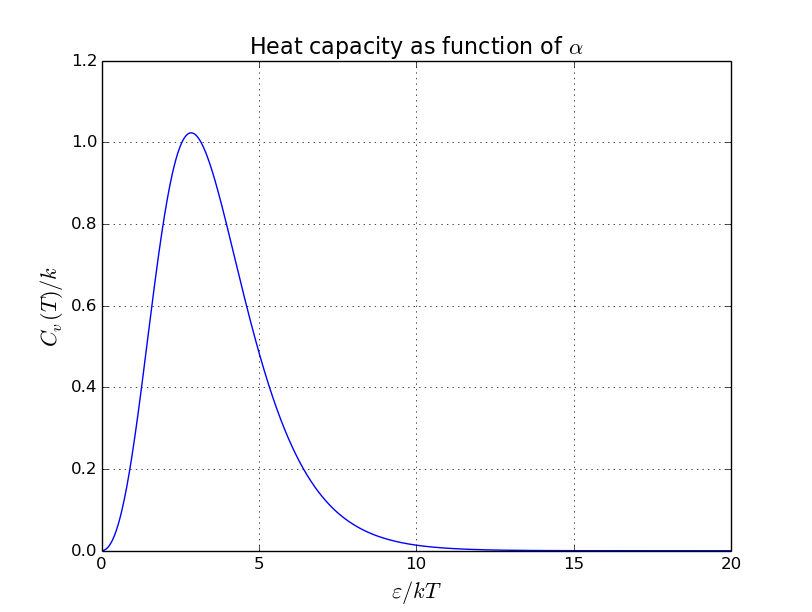
\includegraphics[width=120mm]{oblig2_1.png}
\caption{The heat capacity plotted as a function of $\epsilon/kT$ (dimension less variables) \label{overflow}}
\end{figure}
\textit{The program is found in Appendix A}

\section*{Part II}
In Part II we are looking at rotation of a single diatomic molecule with high energy.
 
\subsection*{d)}
For high temperatures, we need to include degeneration (for low temperatures we do not have degeneration), and in our case the degeneracy is given by 
\begin{equation}
g(j)=2j+1
\end{equation}
The partition function is then
\begin{equation}
Z_R=\sum_j g(j) e^{-\epsilon_j/kT}
\end{equation}
Where $\epsilon_j$ are the energies $\epsilon(j)=j(j+1)\theta_rk$. We obtain
\begin{equation}
\underline{Z_R= \sum_{j=0}^\infty (2j+1)e^{-j(j+1)\theta_r/T}}
\end{equation}
Where I assume that the $k$ which is included in $\epsilon_j$ is Boltzmann's constant.

\subsection*{e)}
Here I will plot the terms $z(j)$ as function of $j$ for different $T$-values. I decided to plot for 6 different $T$-values, which gives 6 different graphs. You can find the plot in \textit{Figure 2}.\par\vspace{3mm}
\begin{figure}[!htbp]
\centering
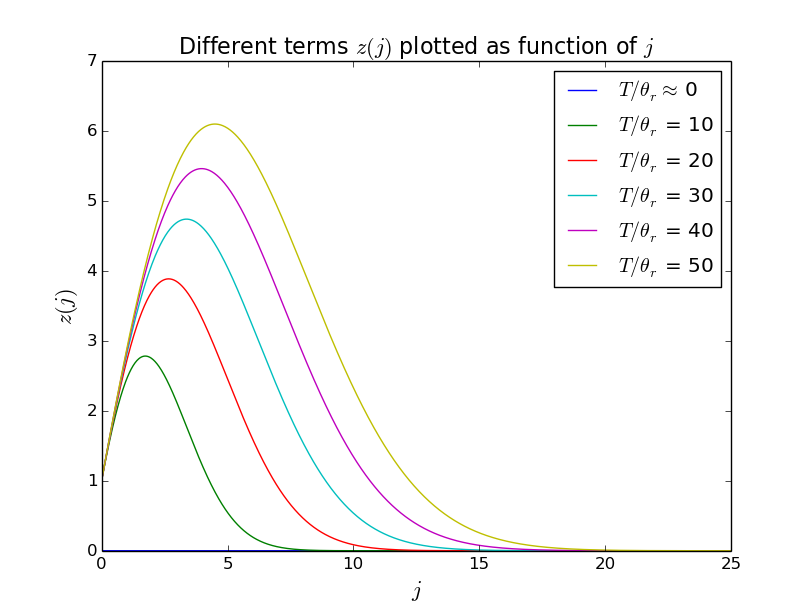
\includegraphics[width=120mm]{oblig2_2.png}
\caption{Different terms $z(j)$ (up to $j=25$) plotted for 6 different $T/\theta_r$-values $T/\theta_r\in [0,50]$. See the text below for more information. \label{overflow}}
\end{figure}
From \textit{Figure 2} we observe 5 different graphs, but why so? I plotted $z(t)$ for 6 different $T/\theta_r$-values, but for $T/\theta_r=10^{-8}$ the graph converges so fast to zero that we can not see it. The smallest value $T/\theta_r=1e-8$ is not chosen to be zero because then we will get a exponent that goes to $-\infty$. In the principle $j$ can only be an integer, but since I want smooth and nice curves, I choose $dj<1$. \par\vspace{3mm}
So, what do the graphs tell us? We know that all the terms in the sum $Z=\sum_jz(j)$ are located on the graph, so when the graph goes to zero, we know that the values of the terms also go to zero. We can therefore read from the graph how many terms there are necessary to include to get a good picture of the sum. \par\vspace{3mm}
An other property of this plot, is that we can estimate $Z_R$ with just looking at the graphs. We know that $Z_R$ is the sum of all the terms, and this is about the same as area under the curve (I could have made a histogram to show this, just like I did in Oblig 01). You are maybe thinking that the area under the graph is the integral, but the integral is just the area of a histogram when the width of the columns goes to zero. In our case this width is 1, but it is still a usable estimate. \par\vspace{3mm}
\textit{The program can be found in Appendix B}

\subsection*{f)}
In the previous exercise I argued for that the sum $Z_R$ could be approximated with an integral, but that is a bit rough estimate. When $T>>\theta_r$, this approximation becomes much better since the exponent stores smaller values and the difference between the $j$'s is small compared with the total number of $j$'s. This can best be explained by a figure (\textit{see Figure 3}).\par\vspace{3mm}
\begin{figure}[!htbp]
\centering
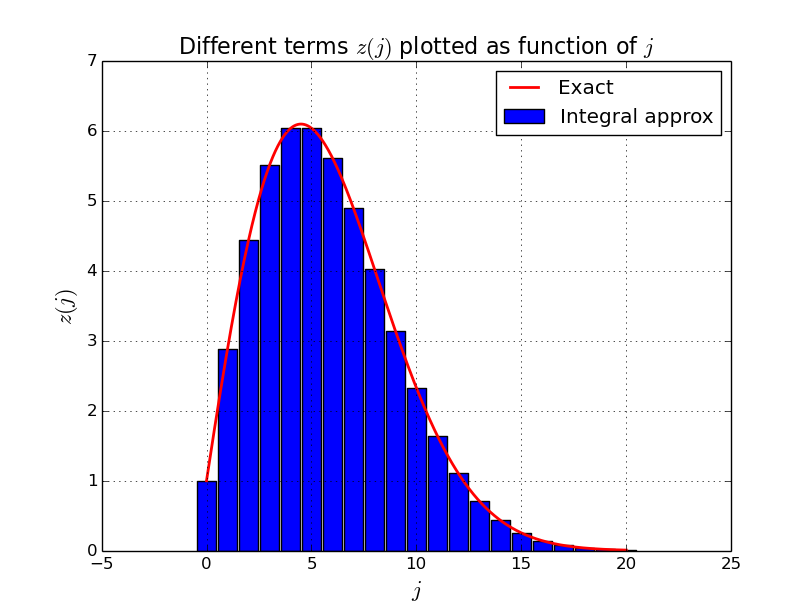
\includegraphics[width=120mm]{oblig2_3.png}
\caption{Different terms $z(j)$ (up to $j=25$) plotted for 6 different $T/\theta_r$-values $T/\theta_r\in [0,50]$. See the text below for more information. \label{overflow}}
\end{figure}
As we can see, the integral approximation is not perfect, but it will overly the exact solution cause the area under the curve is a little bigger than the total area of the histogram. The integral can be written as
\begin{equation}
Z_r\approx \int_0^\infty (2j+1)e^{-j(j+1)\theta_r/T}dj
\end{equation}
To solve this, I need to do a substitution, with for example choosing $u=-j(j+1)\theta_r/T$. This gives $u'=-(2j+1)\theta_r/T$:
$$\Rightarrow -\frac{T}{\theta_r} \int_0^\infty u' e^u dj=-\frac{T}{\theta_r}\int_0^\infty e^udu=-\frac{T}{\theta_r}\bigg[e^{-\infty}-e^0\bigg]=\underline{\frac{T}{\theta_r}}$$
This expression tells us that $Z_r$ is proportional to $T$ (for large $T$'s), and if we go back to the plot in exercise $e)$, we can actually see that this seems to be correct.\par\vspace{3mm}
\textit{The program can be found in Appendix C}

\subsection*{g)}
We are now looking at the case when $T<<\theta_r$, and we can not approximate this to an integral cause the step length will be too big to make a good estimate. Then it is nothing else to than to set up the sum term by term. Fortunately we will see that we do not need many terms to get a good picture of the sum:
$$Z=\sum_{j=0}^\infty (2j+1)e^{-j(j+1)\theta_r/T}=1e^{-0\theta_r/T}+3e^{-2\theta_r/T}+5e^{-6\theta_r/T}...$$
The first term is going to be 1, but the remaining terms will be really small (since we have low temperatures). To keep having a partial function that depends on $T$, we need to keep the second term, no matter if it is small. Our low-temperature approximation is therefore
\begin{equation}
Z_r(T)\approx 1+3e^{-2\theta_r/T}
\end{equation}

\subsection*{h)}
I will again use the expression from Equation (2) to find the energies:
$$E=-\frac{d\ln z}{d\beta}$$
Where $\beta=1/kT$. The partial function for high temperatures expressed with $\beta$ is $Z\approx 1/\theta_rk\beta$, so we can find the energies:
$$E=-\frac{d}{d\beta}\Bigg(\ln\bigg(\frac{1}{\theta_rk\beta}\bigg)\Bigg)=\frac{\theta_r k\beta}{\theta_r k\beta^2}=\frac{1}{\beta}=\underline{kT}$$
Finally we obtain a pretty answer!\par\vspace{3mm}
For low temperatures we have $Z\approx\Big(1+3e^{-2k\theta_r\beta}\Big)$.
$$E=-\frac{d}{d\beta}\bigg(\ln\Big(1+3e^{-2k\theta_r\beta}\Big)\bigg) =\frac{6k\theta_re^{-2k\theta_r\beta}}{1+3e^{-2k\theta_r\beta}}=\underline{\frac{2k\theta_r}{1+1/3e^{2\theta_r/T}}}$$
This is not that pretty, but that is how the nature is.

\subsection*{i)}
I will use the heat capacity formula found in Equation (4) in exercise $c)$. For high temperatures the calculation is really simple:
\begin{equation}
C_v(T)=\frac{d}{dt}(kT)=\underline{k}
\end{equation}
So for high temperatures a diatomic molecule that is in a macroscopic canonical system has heat capacity equal to Boltzmann's constant!\par\vspace{3mm}
For low temperatures, we get
\begin{equation}
C_v(T)=\frac{d}{dT}\bigg(\frac{2k\theta_r}{1+1/3e^{2\theta_r/T}}\bigg)=\underline{\frac{4\theta_r^2k}{3T^2}\frac{e^{2\theta_r/T}}{(1+1/3e^{2\theta_r/T})^2}}
\end{equation}
If we set $2\theta_rk=\epsilon$, we have the same expression as we found in exercise $c)$. The reason is that we have low energies in the both cases, and since we have chosen $\epsilon$ to be an arbitrary energy unit, we should get a expression on the same form. 

\subsection*{j)}
When we make programs which calculate the partition function, we have to remember that we are doing an approximation since we are not able to include a infinity number of terms. We cannot ensure that the terms are converging to zero, but when a term is about one thousandth of the largest term, the approximation should be good enough. I could have done this with an if-test or a while loop, but by looking at \textit{Figure 2}, I can decide how many term that I need to include. For instance, if we have $(T/\theta_r)_{max}=10$, we can read from the figure that we need about 8-10 terms to make a good approximation. I think the program becomes much more transparent with a plain for-loop instead of a while-loop with if-tests, so I do this the manual way.
\begin{lstlisting}
#--Constants--
J=10                            # Number of terms in Z
T = np.linspace(1e-8,10,1000)   # Actually T/Theta-values

#--Generate Z with J terms--
def Z(J):
    z=0
    for j in range(J):
	    z += (2*j+1)*np.exp(-j*(j+1)/T)
    return z
\end{lstlisting}
Where I assume that the exponential function exp is already imported. 

\subsection*{k)}
In this exercise I will use the program discussed in exercise $j)$ to plot my approximation of $Z(T,V,N)$ compared with the exact solution. My high-temperature approximation is $Z\approx T/\theta_r$, and the plot can be found in \textit{Figure 4}.
\begin{figure}[!htbp]
\centering
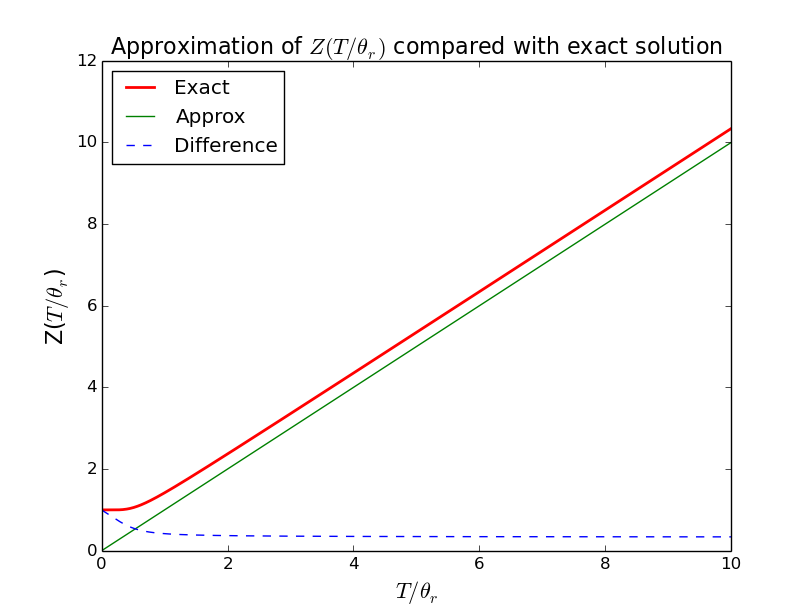
\includegraphics[width=120mm]{oblig2_4.png}
\caption{Here I have plotted approximations with different number of terms with the exact solution. The deviations are included as dashed lines. See text for mote description \label{overflow}}
\end{figure}
From the figure we can see that the differences between the exact and the approximated solutions (the deviations) are decreasing when we include more terms. We can see that the approximation with 10 terms is approach parallel with the exact solution, but if we increase the maximum $T/\theta_r$-value (in other words expanding the plot area) we will see that big deviations will occur for also this approximation. In principle we need to include infinity number of terms if we want the approximation to keep being parallel with the exact solution, but we can make a good approximation for a range of $T/\theta_r$ with relative few terms.\par\vspace{3mm}
\textit{The program can be found in Appendix D}

\subsection*{l)}
If I decide to plot a infinity number of terms with my program from the two previous exercises, we will see that the approximation is still not one hundred percent correct for neither low or high temperatures (something that is actually not possible). For heigh temperatures we can see that the approximate graph is consistent a little above the exact solution, so our high temperature approximation is a little too high. By looking at the differences, we can estimate the deviation as about $1/3$ (No units, the partial function is dimension less). The reason of this is exactly what we saw in exercise $f)$, the area under the approximated graph is simply bigger than the total area of the histogram. 

\subsection*{m)}
So far I have found the energy and heat capacity analytical by derivation, but how to do this on the computer? First I will rewrite the energy expression:
\begin{equation*}
E=-\frac{\partial \ln(Z)}{\partial \beta}=-\frac{\partial \ln(Z)}{\partial (1/kT)}=-k\theta_r\frac{\partial \ln(Z)}{\partial (\theta_r/T)}
\end{equation*}
\begin{equation}
\Rightarrow\quad \frac{E}{k\theta_r}=-\frac{\partial \ln(Z)}{\partial (\theta_r/T)}
\end{equation}
Now I have a expression which depends on $\theta_r/T$, the inverse of the variable I have been working with in almost all the exercises. The clue now is to observe that the derivative is just the difference between all the elements in a list, so Equation (13) can be written as  
\begin{equation*}
\frac{E}{k\theta_r}=-\frac{diff \ln(Z)}{diff (\theta_r/T)}
\end{equation*}
Where for example 
$$diff(T^{-1})=\bigg[\Big(T_2^{-1}-T_1^{-1}\Big),\Big(T_3^{-1}-T_2^{-1}\Big),...,\Big(T_N^{-1}-T_{N-1}^{-1}\Big)\bigg]$$ 
We have to take care of that the diff-lists are one element shorter than the original lists, so actually we need to find the midpoint between all the elements and store them into a list. This can be done by this script:
\begin{lstlisting}
new_T=np.zeros(len(T)-1)
for i in range(len(T)-1):
	new_T[i]=(T[i+1]-T[i])/2.
\end{lstlisting}
The numpy library in python has a function \textit{diff} which transforms a list $L$ into \textit{diff(L)}. I will do the same with the heat capacity, which is still given by
$$C_v(T)=\bigg(\frac{\partial E'}{\partial T}\bigg)_{N,V}$$
Since we are going to send in $E'=E/k\theta_r$, we can make the expression dimension less:
$$\frac{C_v(T)}{k}=\frac{\partial E}{\partial T/\theta_r}$$
so the program will looks like this:
\begin{lstlisting}
#--Energy--
def E(T,Z):
    invT = 1./T
    lnZ_list = np.log(Z)

    diff_invT = np.diff(invT)
    print diff_invT
    diff_lnZ = np.diff(lnZ_list)
    return -diff_lnZ/diff_invT

E = E(T,Z(J))

#--Heat Capacity--
def Cv(E,T):
    diff_E = np.diff(E)
    diff_T = np.diff(T)
    return diff_E/diff_T[0:-1]
\end{lstlisting}
Where I assume that the Z-list is given (for example from my program in exercise $j)$). 

\subsection*{n)}
I choose my largest $T/\theta_r$-value as 10, so there is enough to include 10 terms(see exercise $l)$). By plotting the energy and heat capacity found in the previous exercise, I obtain the plots in \textit{Figure 5} and \textit{6}.
\begin{figure}[H]
\centering
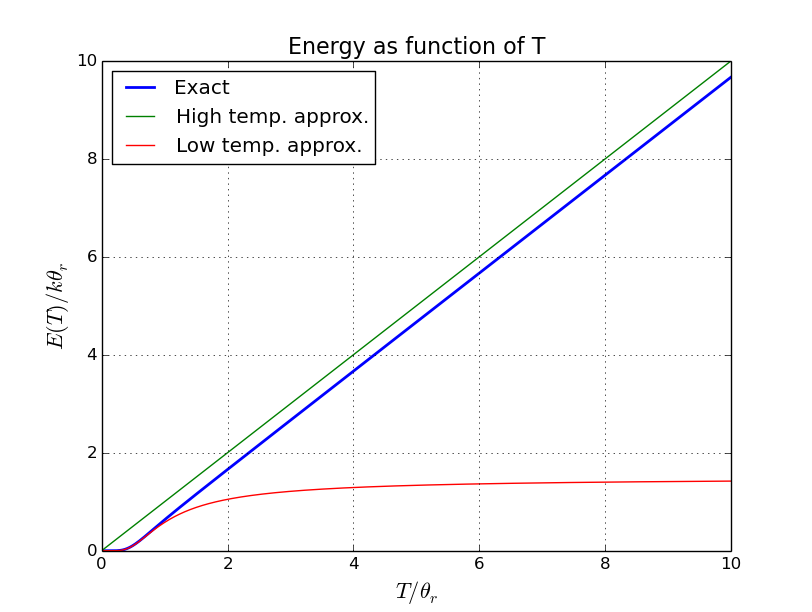
\includegraphics[width=120mm]{oblig2_5.png}
\caption{The exact energy plotted as function of $T/\theta_r$, compared with the low- and high energy approximations \label{overflow}}
\end{figure}
\begin{figure}[H]
\centering
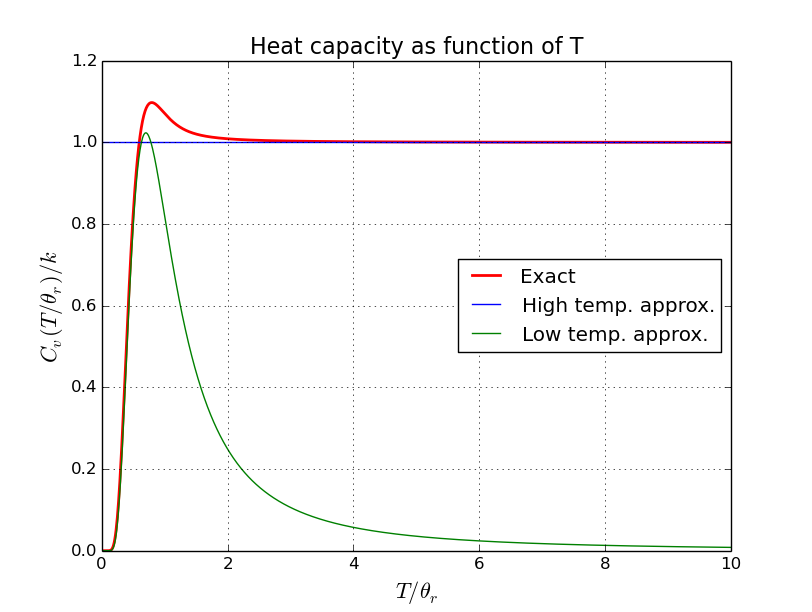
\includegraphics[width=120mm]{oblig2_6.png}
\caption{The exact heat capacity plotted as function of $T/\theta_r$, compared with the low- and high heat capacity approximations \label{overflow}}
\end{figure}
I found that the high temperature estimation of energy is $kT$, but since I am plotting $E/k$, the high temperature estimation line is diagonal. From \textit{Figure 5} we can see that the low temperature approximation is good until $T/\theta_r\approx 1$, and the high temperature approximation is a little too high when the temperature is high.\par\vspace{3mm}
For the heat capacity, we can see that the high temperature approximation is good when $T/\theta_r>2$, and the low temperature approximation is good for $T/\theta_r<1$. I found that the high temperature approximation of the heat capacity was $k$, but since we are plotting $C_v(T/\theta_r)/k$ as function of $T/\theta_r$, this is simply 1.\par\vspace{3mm}
\textit{See Appendix E for the script}

\newpage
\section*{Code attachment}
\subsection*{Appendix A}
\lstinputlisting[language=Python]{oblig02_c.py}

\subsection*{Appendix B}
\lstinputlisting[language=Python]{oblig02_e.py}

\subsection*{Appendix C}
\lstinputlisting[language=Python]{oblig02_f.py}

\subsection*{Appendix D}
\lstinputlisting[language=Python]{oblig02_j.py}

\subsection*{Appendix E}
\lstinputlisting[language=Python]{oblig02_m.py}

\end{document}